\chapter{细胞：生命的共同单位}\label{ch:g10:cells-common-unit}

用棉签刮取口腔内侧，把刮下的物质涂在载玻片上，
滴一滴蓝色染料，用显微镜以四百倍观察：
可以看到一片扁平、形状不规则的“瓦片”，每块都在
靠近中心处有一个颜色较深的斑点。剥取洋葱鳞片内侧的薄表皮，
再次观察，可见整齐排列的长方形“砖块”，每块也都有自己的斑点。池塘水中
可以看到椭圆形的生物，周身有一圈纤毛，划动着游过。这三种样本
在肉眼看来毫无共同之处。在显微镜下，它们都
由同一种物体——\omterm{def:g10:cells-common-unit:cell}{细胞}——构成。本章讨论
这种物体是什么、如何被观察，以及为什么一切生物都由它构成。

\section{细胞学说}

\begin{definition}[细胞]\label{def:g10:cells-common-unit:cell}
称\emph{细胞}\index{细胞}为生物中能够独立存活的最小单位：一团含水的
内容物，即
\emph{细胞质}\index{细胞质}，外面包有一层薄薄的
\emph{质膜}\index{质膜}，它把细胞与
外界隔开，同时允许选择性的物质通过。细胞
摄取物质和能量，加以转化，
使其生长，并分裂为两个细胞。
\end{definition}

\begin{proposition}[细胞学说]\label{prop:g10:cells-common-unit:theory}
以下三条陈述由十九世纪的显微镜观察确立，
共同构成\omterm{def:g10:cells-common-unit:cell}{细胞}学说：
\begin{enumerate}
  \item 每种生物都由一个或多个\omterm{def:g10:cells-common-unit:cell}{细胞}构成；
  \item \omterm{def:g10:cells-common-unit:cell}{细胞}是生物结构和功能的基本单位——
        比\omterm{def:g10:cells-common-unit:cell}{细胞}更小的部分单独都不具有生命；
  \item 每个\omterm{def:g10:cells-common-unit:cell}{细胞}都来自已存在的\omterm{def:g10:cells-common-unit:cell}{细胞}，通过分裂产生。
\end{enumerate}
\end{proposition}
\begin{proof}[证据]
第一条的依据是对植物（施莱登，
1838）和动物（施旺，1839）的系统考察，所用显微镜经过改进；
所检查的每种组织，无论外观如何不同，都能分辨出\omterm{def:g10:cells-common-unit:cell}{细胞}。
第三条由菲尔绍（1855）确立，并依靠对
生长组织中分裂\omterm{def:g10:cells-common-unit:cell}{细胞}的观察；另一种设想——\omterm{def:g10:cells-common-unit:cell}{细胞}由
液体中自发形成——从未被观察到，而巴斯德的
微生物实验（在\cref{ch:g11:antibiotic-resistance}中
再次讨论）终结了这一问题。第二条由第一条
推出，并基于这一事实：分离出的\omterm{def:g10:cells-common-unit:cell}{细胞}
置于合适的液体中仍能存活，而\omterm{def:g10:cells-common-unit:cell}{细胞}的任何碎片则不能。
\end{proof}

\begin{example}[单细胞还是多细胞]\label{ex:g10:cells-common-unit:onemany}
酵母、草履虫或细菌都是单个\omterm{def:g10:cells-common-unit:cell}{细胞}，能完成
一切功能——取食、运动、分裂。橡树或人则是
由多种\omterm{def:g10:cells-common-unit:cell}{细胞}组成的协作体，每种\omterm{def:g10:cells-common-unit:cell}{细胞}各承担一部分工作：人体
约含 $\num{3e13}$ 个\omterm{def:g10:cells-common-unit:cell}{细胞}，分属约两百种类型。两者之间
是群体和简单的多\omterm{def:g10:cells-common-unit:cell}{细胞}生物，
但没有任何生物是由
\omterm{def:g10:cells-common-unit:cell}{细胞}以外的东西构成的。
\end{example}

\section{观察细胞：尺度与显微镜}

\begin{definition}[放大率与分辨率]\label{def:g10:cells-common-unit:magnification}
仪器的\emph{放大率}\index{放大率}，是像的大小与
物体大小之比。其\emph{分辨率}\index{分辨率}，是
仪器仍能分辨为相互分开的
两点之间的最小距离。若放大图像超出分辨率所允许的范围，
放大的只是模糊，而不是细节。
\end{definition}

\begin{proposition}[两种仪器，两种尺度]\label{prop:g10:cells-common-unit:microscopes}
光学显微镜的放大倍数可达约 $\times 1500$，\omterm{def:g10:cells-common-unit:magnification}{分辨率}约为
\qty{0.2}{\micro m}：可以显示\omterm{def:g10:cells-common-unit:cell}{细胞}、\omterm{def:g10:cells-common-unit:organelle}{细胞核}、
\omterm{def:g10:cells-common-unit:organelle}{叶绿体}和细菌，且为彩色活体。电子显微镜不用光，而是用
电子束：\omterm{def:g10:cells-common-unit:magnification}{分辨率}低于
\qty{1}{nm}，放大倍数可达 $\times 10^6$；它能揭示\omterm{def:g10:cells-common-unit:cell}{细胞}的内部
结构——膜、\omterm{def:g10:cells-common-unit:organelle}{线粒体}、\omterm{def:g10:cells-common-unit:organelle}{核糖体}，甚至
大分子——但观察的样本已死亡、干燥，并切成
薄于一微米的薄片。
\end{proposition}
\admitted

\begin{omfigure}
\begin{tikzpicture}[>=Stealth]
  % log scale ruler from 1 nm (0) to 1 m (9 decades), 1.3 cm per decade
  \draw[thick] (0,0) -- (11.7,0);
  \foreach \d/\t in {0/{\qty{1}{nm}}, 1/{\qty{10}{nm}}, 2/{\qty{100}{nm}},
      3/{\qty{1}{\micro m}}, 4/{\qty{10}{\micro m}}, 5/{\qty{100}{\micro m}},
      6/{\qty{1}{mm}}, 7/{\qty{1}{cm}}, 8/{\qty{10}{cm}}, 9/{\qty{1}{m}}}
    \draw (1.3*\d,0.12) -- (1.3*\d,-0.12) node[below, font=\scriptsize] {\t};
  % objects above the ruler
  \foreach \d/\h/\t in {0.3/0.5/{DNA 宽度}, 0.9/1.1/{蛋白质},
      2.0/0.5/{病毒}, 3.0/1.1/{细菌}, 4.3/0.5/{动物细胞},
      4.9/1.1/{植物细胞}, 6.0/0.5/{蛙卵}, 6.9/1.1/{蚂蚁},
      8.3/0.5/{人}}
    \node[font=\scriptsize, anchor=south] at (1.3*\d,\h) {\t};
  \foreach \d in {0.3,0.9,2.0,3.0,4.3,4.9,6.0,6.9,8.3}
    \fill (1.3*\d,0) circle (1.6pt);
  \foreach \d/\h in {0.9/1.1,3.0/1.1,4.9/1.1,6.9/1.1}
    \draw[gray] (1.3*\d,0.05) -- (1.3*\d,\h);
  \foreach \d/\h in {0.3/0.5,2.0/0.5,4.3/0.5,6.0/0.5,8.3/0.5}
    \draw[gray] (1.3*\d,0.05) -- (1.3*\d,\h);
  % instrument ranges below
  \draw[<->, omDef, thick] (0,-1.0) -- (3.9,-1.0)
    node[midway, below, font=\scriptsize, omDef] {电子显微镜};
  \draw[<->, omProp, thick] (2.6,-1.6) -- (6.5,-1.6)
    node[midway, below, font=\scriptsize, omProp] {光学显微镜};
  \draw[<->, omMeth, thick] (5.9,-2.2) -- (11.7,-2.2)
    node[midway, below, font=\scriptsize, omMeth] {肉眼};
\end{tikzpicture}

{\small 对数刻度下的尺寸：每一级都比前一级大十倍。
肉眼的分辨能力约为 \qty{0.1}{mm}；光学显微镜可达
\qty{0.2}{\micro m}，可以看到完整的\omterm{def:g10:cells-common-unit:cell}{细胞}和细菌；电子
显微镜可分辨至纳米量级，并显示内部的各部分。}
\end{omfigure}

\begin{method}[在显微照片上测量物体]\label{met:g10:cells-common-unit:measure}
显微照片上标注有放大倍数或比例尺。
\begin{enumerate}
  \item 有比例尺时：测量比例尺（图上长 \qty{12}{mm}，
        标注为 \qty{10}{\micro m}）和物体（\qty{30}{mm}）；
        实际长度为 $30 \times 10/12 =
        \qty{25}{\micro m}$。
  \item 有放大倍数时：实际长度 $=$ 图上测得的长度除以放大倍数；
        图中长 \qty{20}{mm} 的\omterm{def:g10:cells-common-unit:cell}{细胞}（放大 $\times 400$ 时）
        实际长度为 $20/400 = \qty{0.05}{mm} = \qty{50}{\micro m}$。
  \item 始终写明单位，并进行换算：$\qty{1}{mm} =
        \qty{1000}{\micro m}$，$\qty{1}{\micro m} = \qty{1000}{nm}$。
\end{enumerate}
\end{method}

\begin{example}[口腔上皮细胞]\label{ex:g10:cells-common-unit:cheek}
在 $\times 400$ 的图像中测得一个口腔上皮\omterm{def:g10:cells-common-unit:cell}{细胞}宽 \qty{24}{mm}，实际宽度为
$24/400 = \qty{0.06}{mm} = \qty{60}{\micro m}$，其\omterm{def:g10:cells-common-unit:organelle}{细胞核}
图中长 \qty{3}{mm}，约为 \qty{8}{\micro m}。红\omterm{def:g10:cells-common-unit:cell}{细胞}为 \qty{7}{\micro m}；
口腔中的细菌长 \qty{1}{\micro m}，在相同放大倍数下
仅能勉强分辨为小点。
\end{example}

\section{细胞内部}

\begin{definition}[细胞器]\label{def:g10:cells-common-unit:organelle}
\emph{细胞器}\index{细胞器}是位于\omterm{def:g10:cells-common-unit:cell}{细胞}内部的一种结构，
由自身的膜包围，执行特定的功能。主要的\omterm{def:g10:cells-common-unit:cell}{细胞}器
包括以下几种：
\begin{itemize}
  \item \emph{细胞核}\index{细胞核}，含有染色体——
        即\cref{ch:g10:universal-dna}中的 DNA——并
        控制\omterm{def:g10:cells-common-unit:cell}{细胞}的活动；
  \item \emph{线粒体}\index{线粒体}，部分长约
        \qty{1}{\micro m}，有机分子在其中与氧气
        结合而被分解，释放可利用的能量（\omterm{def:g10:cells-common-unit:cell}{细胞}呼吸，
        在\cref{ch:g10:cell-metabolism}中）；
  \item 植物\omterm{def:g10:cells-common-unit:cell}{细胞}中的\emph{叶绿体}\index{叶绿体}，
        含叶绿素而呈绿色，是进行光合作用的场所，以及一个
        充满水的大型\emph{液泡}\index{液泡}，使
        \omterm{def:g10:cells-common-unit:cell}{细胞}保持挺实。
\end{itemize}
在\omterm{def:g10:cells-common-unit:cell}{质膜}外，植物\omterm{def:g10:cells-common-unit:cell}{细胞}还包被着一层坚硬的
\emph{细胞壁}\index{细胞壁}，由纤维素构成；动物\omterm{def:g10:cells-common-unit:cell}{细胞}没有。
每个\omterm{def:g10:cells-common-unit:cell}{细胞}的\omterm{def:g10:cells-common-unit:cell}{细胞质}中还含有数以百万计的
\emph{核糖体}\index{核糖体}，是约 \qty{25}{nm} 的颗粒，
负责合成\omterm{def:g10:chemistry-of-life:families}{蛋白质}，只有用电子显微镜才能看到。
\end{definition}

\begin{omfigure}
\begin{tikzpicture}[>=Stealth, font=\small, line cap=round, line join=round]
  % ---------- animal cell ----------
  \begin{scope}
    \draw[thick, fill=omDef!6] (0,0) .. controls (1.4,1.9) and (2.9,0.9) .. (2.4,-0.2)
      .. controls (2.1,-1.5) and (0.6,-2.0) .. (-0.6,-1.6)
      .. controls (-2.4,-1.1) and (-2.6,0.6) .. (-1.4,1.3)
      .. controls (-0.9,1.6) and (-0.5,1.4) .. (0,0) -- cycle;
    % nucleus with nucleolus
    \draw[thick, fill=omDef!30] (-0.4,-0.1) circle (0.72);
    \fill[omDef!70] (-0.55,0.05) circle (0.17);
    \node[font=\scriptsize] at (-0.4,-0.33) {细胞核};
    % mitochondria with cristae
    \foreach \x/\y/\r in {1.3/0.4/25, 1.1/-0.9/-35, -1.5/-0.9/60, 0.5/0.9/-10} {
      \begin{scope}[rotate around={\r:(\x,\y)}]
        \draw[fill=omProp!35] (\x,\y) ellipse (0.36 and 0.17);
        \draw[omProp!80!black, thin] (\x-0.2,\y-0.1) -- (\x-0.2,\y+0.1) (\x-0.07,\y-0.12) -- (\x-0.07,\y+0.12) (\x+0.07,\y-0.12) -- (\x+0.07,\y+0.12) (\x+0.2,\y-0.1) -- (\x+0.2,\y+0.1);
      \end{scope}}
    % ribosomes
    \foreach \x/\y in {0.5/-1.2, -1.6/0.5, 0.9/0.0, -1.3/-0.5, 1.9/-0.4, 0.2/1.2, -0.9/0.9, 1.6/1.0, -0.2/-1.3}
      \fill (\x,\y) circle (1.1pt);
    \node[anchor=north, font=\small\bfseries] at (0,-2.1) {动物细胞};
    \draw[->] (2.8,1.5) node[right, font=\scriptsize] {质膜} -- (2.35,0.55);
    \draw[->] (2.8,-1.1) node[right, font=\scriptsize] {线粒体} -- (1.5,-0.95);
    \draw[->] (2.8,0.3) node[right, font=\scriptsize] {细胞质} -- (1.85,-0.25);
  \end{scope}
  % ---------- plant cell ----------
  \begin{scope}[xshift=8.3cm]
    % cellulose wall (thick, pale green) and the membrane just inside it
    \draw[line width=4pt, green!35!black!45, fill=omMeth!10, rounded corners=5pt] (-2.4,-1.8) rectangle (2.4,1.8);
    \draw[thick, black!80, rounded corners=4pt] (-2.22,-1.62) rectangle (2.22,1.62);
    % large central vacuole
    \draw[thick, fill=cyan!8, rounded corners=15pt] (-0.95,-1.05) rectangle (1.95,1.15);
    \node[font=\scriptsize] at (0.5,0.1) {液泡};
    % nucleus pressed against the wall, with nucleolus
    \draw[thick, fill=omDef!30] (-1.5,0.8) circle (0.62);
    \fill[omDef!70] (-1.7,1.05) circle (0.14);
    \node[font=\scriptsize] at (-1.5,0.68) {细胞核};
    % chloroplasts: lens-shaped, with stacked membranes inside
    \foreach \x/\y/\r in {-1.55/-0.55/75, -0.35/-1.33/0, 1.05/-1.33/0, 0.25/1.38/0, 1.55/1.38/0} {
      \begin{scope}[rotate around={\r:(\x,\y)}]
        \draw[fill=green!55!black!45] (\x,\y) ellipse (0.36 and 0.18);
        \draw[green!25!black, line width=0.9pt] (\x-0.2,\y-0.06) -- (\x-0.2,\y+0.06) (\x-0.08,\y-0.09) -- (\x-0.08,\y+0.09) (\x+0.06,\y-0.09) -- (\x+0.06,\y+0.09) (\x+0.19,\y-0.06) -- (\x+0.19,\y+0.06);
      \end{scope}}
    % mitochondria
    \foreach \x/\y/\r in {-1.75/-1.2/35, -0.75/1.38/0} {
      \begin{scope}[rotate around={\r:(\x,\y)}]
        \draw[fill=omProp!35] (\x,\y) ellipse (0.3 and 0.14);
        \draw[omProp!80!black, thin] (\x-0.14,\y-0.08) -- (\x-0.14,\y+0.08) (\x,\y-0.1) -- (\x,\y+0.1) (\x+0.14,\y-0.08) -- (\x+0.14,\y+0.08);
      \end{scope}}
    % ribosomes in the thin cytoplasm
    \foreach \x/\y in {-1.1/-1.4, 2.08/0.3, 2.08/-0.8, -2.05/0.1, 0.8/1.42, -2.05/-0.9}
      \fill (\x,\y) circle (1.1pt);
    \node[anchor=north, font=\small\bfseries] at (0,-2.1) {植物细胞};
    \draw[->] (2.8,1.7) node[right, font=\scriptsize] {细胞壁} -- (2.45,1.4);
    \draw[->] (2.8,0.9) node[right, font=\scriptsize] {质膜} -- (2.24,0.7);
    \draw[->] (2.8,-0.3) node[right, font=\scriptsize] {细胞质} -- (2.1,-0.55);
    \draw[->] (2.8,-1.3) node[right, font=\scriptsize] {叶绿体} -- (1.42,-1.33);
  \end{scope}
\end{tikzpicture}

{\small 示意两个\omterm{def:g10:cells-common-unit:prokaryote}{真核细胞}。二者都有膜、
\omterm{def:g10:cells-common-unit:cell}{细胞质}、带橙色的\omterm{def:g10:cells-common-unit:organelle}{线粒体}和\omterm{def:g10:cells-common-unit:organelle}{细胞核}；植物\omterm{def:g10:cells-common-unit:cell}{细胞}另有
纤维素\omterm{def:g10:cells-common-unit:organelle}{细胞壁}、绿色的\omterm{def:g10:cells-common-unit:organelle}{叶绿体}和一个大的中央\omterm{def:g10:cells-common-unit:organelle}{液泡}。
两图均未按比例绘制：真实的\omterm{def:g10:cells-common-unit:organelle}{细胞核}约为\omterm{def:g10:cells-common-unit:cell}{细胞}宽度的十分之一，
\omterm{def:g10:cells-common-unit:organelle}{线粒体}则比\omterm{def:g10:cells-common-unit:cell}{细胞}小一百倍。}
\end{omfigure}

\begin{definition}[原核生物与真核生物]\label{def:g10:cells-common-unit:prokaryote}
DNA 被\omterm{def:g10:cells-common-unit:organelle}{细胞核}包裹的\omterm{def:g10:cells-common-unit:cell}{细胞}，称为
\emph{真核细胞}\index{真核细胞}：动物、植物、真菌
和许多单\omterm{def:g10:cells-common-unit:cell}{细胞}生物都是真核生物。
\emph{原核细胞}\index{原核细胞}没有\omterm{def:g10:cells-common-unit:organelle}{细胞核}，也没有
膜包围的\omterm{def:g10:cells-common-unit:organelle}{细胞器}：其 DNA 游离于\omterm{def:g10:cells-common-unit:cell}{细胞质}中，
大小约为 \qty{1}{\micro m}，外面包有一层
特有的壁。细菌属于原核生物。
\end{definition}

\begin{example}[读一张细菌图]\label{ex:g10:cells-common-unit:bacterium}
肠道细菌 \emph{Escherichia coli} 的电子显微照片
显示一个长 \qty{2}{\micro m}、宽 \qty{0.5}{\micro m} 的杆状\omterm{def:g10:cells-common-unit:cell}{细胞}：
有\omterm{def:g10:cells-common-unit:organelle}{细胞壁}、紧贴壁内的膜、颗粒状的\omterm{def:g10:cells-common-unit:cell}{细胞质}，其中
布满\omterm{def:g10:cells-common-unit:organelle}{核糖体}，中央颜色较浅的区域内，
有单个环状 DNA 分子。没有\omterm{def:g10:cells-common-unit:organelle}{细胞核}，也没有\omterm{def:g10:cells-common-unit:organelle}{线粒体}。然而，该\omterm{def:g10:cells-common-unit:cell}{细胞}取食、生长，
并在丰富的营养液中每二十分钟分裂一次：一切\omterm{def:g10:cells-common-unit:cell}{细胞}学说所要求的，
都具备于体积仅为一个颊\omterm{def:g10:cells-common-unit:cell}{细胞}千分之一的\omterm{def:g10:cells-common-unit:cell}{细胞}之中。
\end{example}

\begin{omfigure}
\begin{tikzpicture}
  \node[anchor=south west, inner sep=0] (img) at (0,0)
    {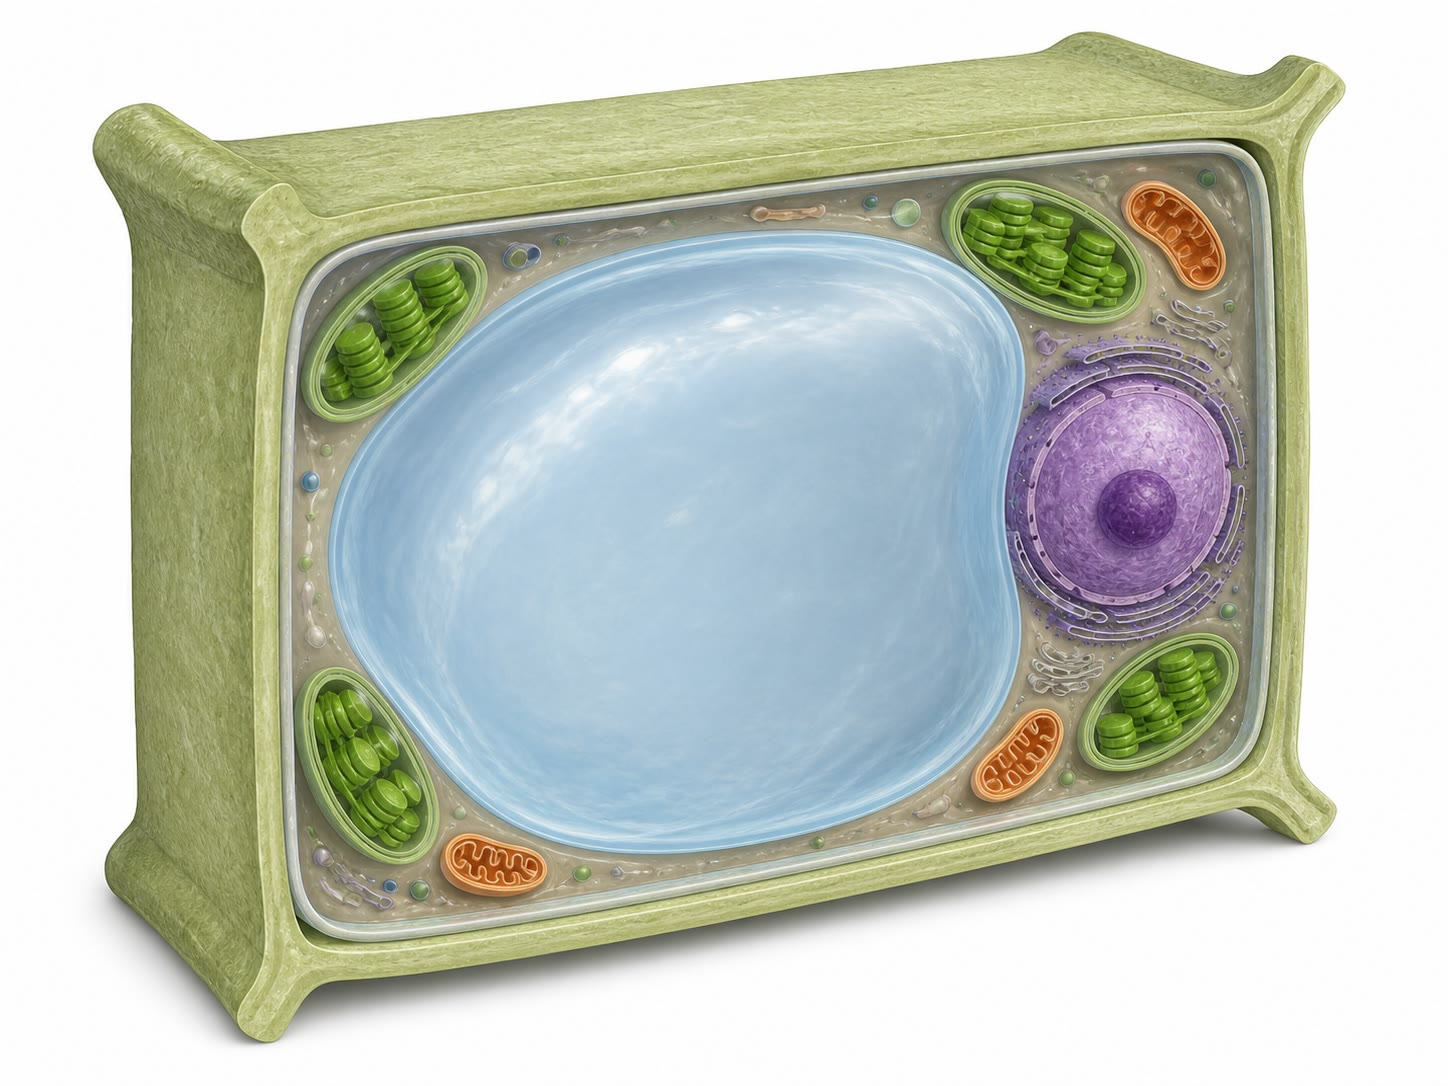
\includegraphics[width=0.52\linewidth]{images/book2/ai/fig-plant-cell-cutaway-v2.jpg}};
  \begin{scope}[x={(img.south east)}, y={(img.north west)},
      every node/.style={font=\small}]
    \draw[omDef, thick] (0.78,0.54) -- (1.05,0.62) node[right] {细胞核};
    \draw[omDef, thick] (0.92,0.28) -- (1.05,0.18) node[right] {细胞壁};
    \draw[omDef, thick] (0.45,0.54) -- (0.45,1.06) node[above] {液泡};
    \draw[omDef, thick] (0.215,0.50) -- (-0.05,0.64) node[left] {质膜};
    \draw[omDef, thick] (0.25,0.30) -- (-0.05,0.30) node[left] {叶绿体};
    \draw[omDef, thick] (0.34,0.21) -- (-0.05,0.08) node[left] {线粒体};
  \end{scope}
\end{tikzpicture}

{\small 剖开的植物\omterm{def:g10:cells-common-unit:cell}{细胞}：坚硬的\omterm{def:g10:cells-common-unit:organelle}{细胞壁}、紧贴其内的\omterm{def:g10:cells-common-unit:cell}{质膜}、
\omterm{def:g10:cells-common-unit:organelle}{细胞核}、绿色的\omterm{def:g10:cells-common-unit:organelle}{叶绿体}，以及
占据大部分体积的\omterm{def:g10:cells-common-unit:organelle}{液泡}。}
\end{omfigure}

\section{细胞众多，形态各异：分化}

\begin{proposition}[分化的细胞]\label{prop:g10:cells-common-unit:specialised}
在多\omterm{def:g10:cells-common-unit:cell}{细胞}生物体中，各类\omterm{def:g10:cells-common-unit:cell}{细胞}共享相同的基本结构和
相同的 DNA，但每类\omterm{def:g10:cells-common-unit:cell}{细胞}的形态和结构都与其功能相适应：
功能：神经元伸出一根长达一米的纤维以传递信号；
红\omterm{def:g10:cells-common-unit:cell}{细胞}失去了\omterm{def:g10:cells-common-unit:organelle}{细胞核}，是扁平的圆盘状，内含大量
血红蛋白；肌纤维是充满收缩
蛋白的巨大\omterm{def:g10:cells-common-unit:cell}{细胞}；根毛是一根细管，用以增大
吸收水分的表面积；叶片的保卫\omterm{def:g10:cells-common-unit:cell}{细胞}改变形状以开启或关闭
气孔。分化取决于共享的基本结构中哪些部分
得以发育。
\end{proposition}
\admitted

\begin{example}[表面积与体积]\label{ex:g10:cells-common-unit:surface}
\omterm{def:g10:cells-common-unit:cell}{细胞}为什么如此之小？\omterm{def:g10:cells-common-unit:cell}{细胞}吸收和排出的一切物质都要穿过
\omterm{def:g10:cells-common-unit:cell}{细胞}膜，其面积随尺寸的平方增长，而
需求则随体积即立方增长。边长为
\qty{10}{\micro m} 的立方体\omterm{def:g10:cells-common-unit:cell}{细胞}，表面积为 \qty{600}{\micro m^2}，
体积为 \qty{1000}{\micro m^3}：每立方微米的膜面积为 \qty{0.6}{\micro m^2}。
边长为 \qty{100}{\micro m} 时，此比值降至
\qty{0.06}{\micro m^2}，每单位内容物的膜面积少了十倍。
大的\omterm{def:g10:cells-common-unit:cell}{细胞}，中心将因缺乏物质交换而
缺乏养料；大的\omterm{def:g10:cells-common-unit:cell}{细胞}（如蛙卵、肌纤维）要么主要为惰性储备物，要么
拉长成细长形，使任何一点都离表面不远。
\end{example}

\begin{omfigure}
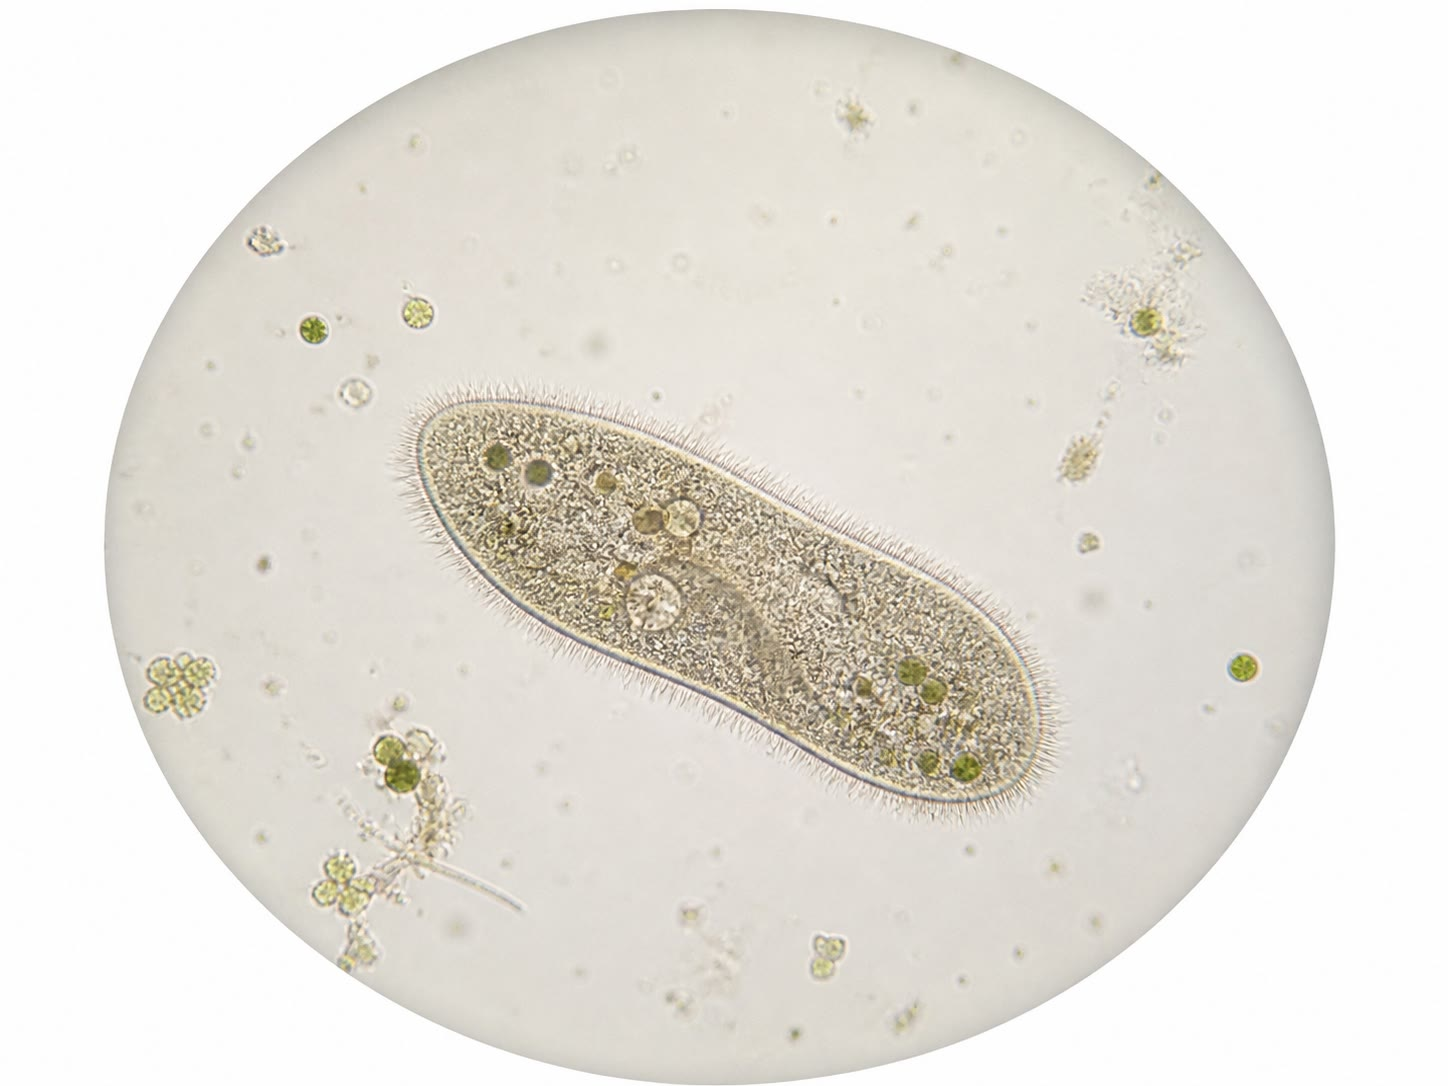
\includegraphics[width=0.62\linewidth]{images/book2/ai/g10-cells-paramecium.jpg}

{\small 池塘水滴在光学显微镜下：一只草履虫，
是一个长四分之一毫米的单\omterm{def:g10:cells-common-unit:cell}{细胞}，
靠数千根微小纤毛的摆动划过绿藻。一个\omterm{def:g10:cells-common-unit:cell}{细胞}，即一个完整的
生物体。}
\end{omfigure}

\begin{remark}[作为开口系统的细胞]\label{rem:g10:cells-common-unit:open}
\omterm{def:g10:cells-common-unit:cell}{细胞}不是密封的袋子。水、氧气、葡萄糖和离子不断穿过其
\omterm{def:g10:cells-common-unit:cell}{细胞}膜，废物也以同样方式排出；把颊\omterm{def:g10:cells-common-unit:cell}{细胞}
置于纯水中，几分钟内便膨胀破裂，置于
浓盐水中则皱缩。\omterm{def:g10:cells-common-unit:cell}{细胞}膜对进出物质的控制
是本科一年级分册的内容；这里只需记住，
\omterm{def:g10:cells-common-unit:cell}{细胞}依靠与外界的交换而生存，交换停止时便
死亡。
\end{remark}

\section{练习}

\begin{exercise}[$\star$]\label{exo:g10:cells-common-unit:1}
写出\omterm{def:g10:cells-common-unit:cell}{细胞}学说的三条内容。
\end{exercise}

\begin{exercise}[$\star$]\label{exo:g10:cells-common-unit:2}
换算：\qty{0.05}{mm} 化为微米；\qty{2500}{nm} 化为微米；
\qty{7}{\micro m} 化为毫米。
\end{exercise}

\begin{exercise}[$\star$]\label{exo:g10:cells-common-unit:3}
\omterm{def:g10:cells-common-unit:cell}{细胞}在图中长 \qty{36}{mm}，该图为 $\times 600$ 的放大图像。
求其实际长度。
\end{exercise}

\begin{exercise}[$\star$]\label{exo:g10:cells-common-unit:4}
列举植物\omterm{def:g10:cells-common-unit:cell}{细胞}中有而动物\omterm{def:g10:cells-common-unit:cell}{细胞}中没有的三种结构，以及
所有\omterm{def:g10:cells-common-unit:cell}{细胞}都有的一种结构。
\end{exercise}

\begin{exercise}[$\star$]\label{exo:g10:cells-common-unit:5}
\omterm{def:g10:cells-common-unit:prokaryote}{原核细胞}与\omterm{def:g10:cells-common-unit:prokaryote}{真核细胞}有何区别？
各举一个例子。
\end{exercise}

\begin{exercise}[$\star\star$]\label{exo:g10:cells-common-unit:6}
在一张显微照片上，标有 \qty{5}{\micro m} 的比例尺
长 \qty{15}{mm}；一个\omterm{def:g10:cells-common-unit:organelle}{线粒体}长 \qty{6}{mm}。求
该\omterm{def:g10:cells-common-unit:organelle}{线粒体}的实际长度以及图像的放大倍数。
\end{exercise}

\begin{exercise}[$\star\star$]\label{exo:g10:cells-common-unit:7}
为什么无论放大倍数多大，光学显微镜都无法显示\omterm{def:g10:cells-common-unit:organelle}{核糖体}？
请用
\cref{def:g10:cells-common-unit:magnification} 中的两个词作答。
\end{exercise}

\begin{exercise}[$\star\star$]\label{exo:g10:cells-common-unit:8}
在显微镜下向马铃薯薄片滴加碘液，\omterm{def:g10:cells-common-unit:cell}{细胞}内
出现蓝黑色的椭圆形颗粒。
利用 \cref{ch:g10:chemistry-of-life} 的内容，说明这些颗粒是什么，
以及这表明植物将储备物质储存在何处。
\end{exercise}

\begin{exercise}[$\star\star$]\label{exo:g10:cells-common-unit:9}
洋葱表皮\omterm{def:g10:cells-common-unit:cell}{细胞}有\omterm{def:g10:cells-common-unit:organelle}{细胞核}和\omterm{def:g10:cells-common-unit:organelle}{细胞壁}，但没有\omterm{def:g10:cells-common-unit:organelle}{叶绿体}，而
苔藓叶片的\omterm{def:g10:cells-common-unit:cell}{细胞}里却充满\omterm{def:g10:cells-common-unit:organelle}{叶绿体}。请根据
两种组织各自的生活环境，解释这一差异。
\end{exercise}

\begin{exercise}[$\star\star$]\label{exo:g10:cells-common-unit:10}
计算边长为 \qty{1}{\micro m}（细菌）的立方体\omterm{def:g10:cells-common-unit:cell}{细胞}
与边长为 \qty{20}{\micro m}（典型动物\omterm{def:g10:cells-common-unit:cell}{细胞}）的立方体\omterm{def:g10:cells-common-unit:cell}{细胞}
的表面积与体积之比，并判断哪一种仅靠
通过\omterm{def:g10:cells-common-unit:cell}{细胞}膜的简单扩散即可满足需要？
\end{exercise}

\begin{exercise}[$\star\star$]\label{exo:g10:cells-common-unit:11}
一个细菌在营养丰富的肉汤中每 \qty{20}{min} 分裂一次。从
一个\omterm{def:g10:cells-common-unit:cell}{细胞}开始，\qty{2}{h} 后有多少个\omterm{def:g10:cells-common-unit:cell}{细胞}？\qty{4}{h} 后呢？
\end{exercise}

\begin{exercise}[$\star\star\star$]\label{exo:g10:cells-common-unit:12}
红\omterm{def:g10:cells-common-unit:cell}{细胞}没有\omterm{def:g10:cells-common-unit:organelle}{细胞核}，也没有\omterm{def:g10:cells-common-unit:organelle}{线粒体}。它是否满足
\cref{def:g10:cells-common-unit:cell} 的条件？请讨论，已知它
约能存活 120 天，不能分裂，并且由
骨髓中有\omterm{def:g10:cells-common-unit:organelle}{细胞核}的\omterm{def:g10:cells-common-unit:cell}{细胞}产生。
\end{exercise}

\begin{exercise}[$\star\star\star$]\label{exo:g10:cells-common-unit:13}
1665 年，胡克在一片软木薄片中看到了“\omterm{def:g10:cells-common-unit:cell}{细胞}”——
即带有厚壁的空格子。请用本章的术语解释
他实际看到的是什么，以及他为何不可能在其中看到\omterm{def:g10:cells-common-unit:organelle}{细胞核}。
\end{exercise}

\begin{exercise}[$\star\star\star$]\label{exo:g10:cells-common-unit:14}
病毒是大小为 \qty{20}{nm} 至 \qty{300}{nm} 的颗粒，
含有\omterm{def:g10:chemistry-of-life:families}{核酸}和\omterm{def:g10:chemistry-of-life:families}{蛋白质}，不能独立生长或分裂，
只能在\omterm{def:g10:cells-common-unit:cell}{细胞}内增殖。它们是\omterm{def:g10:cells-common-unit:cell}{细胞}吗？它们是活的吗？
请根据\omterm{def:g10:cells-common-unit:cell}{细胞}学说进行论证。
\end{exercise}

\begin{exercise}[$\star\star\star$]\label{exo:g10:cells-common-unit:15}
一根肌纤维是单个\omterm{def:g10:cells-common-unit:cell}{细胞}，长 \qty{3}{cm}，
宽 \qty{50}{\micro m}，内含数百个\omterm{def:g10:cells-common-unit:organelle}{细胞核}。计算其体积，并与
边长为 \qty{20}{\micro m} 的立方体\omterm{def:g10:cells-common-unit:cell}{细胞}的体积相比较；然后
根据 \cref{ex:g10:cells-common-unit:surface}，解释其形状和众多\omterm{def:g10:cells-common-unit:organelle}{细胞核}
如何使这样的尺寸得以运作。
\end{exercise}

\section{问题：统计人体的细胞数量}

\begin{problem}[{周末问题——一节显微观察课：从载玻片上的洋葱表皮
到人体细胞数目
的估算}]
\label{pb:g10:cells-common-unit:1}
某班级用一个下午在显微镜前进行观察。可用的物镜给出的总放大倍数分别为
$\times 40$、$\times 100$ 和
$\times 400$；在 $\times 100$ 下，视野直径为 \qty{1.8}{mm}。

\medskip
\noindent\textbf{第一部分——洋葱。}
\begin{enumerate}
  \item 在 $\times 100$ 下，视野宽度内约可并排容纳 9 个洋葱\omterm{def:g10:cells-common-unit:cell}{细胞}，
        由此估算单个\omterm{def:g10:cells-common-unit:cell}{细胞}的宽度，单位为
        微米。
  \item 在 $\times 400$ 下，视野宽度缩小为原来的四分之一。
        其宽度是多少？视野中可并排容纳多少个这样的\omterm{def:g10:cells-common-unit:cell}{细胞}？
  \item 一名学生在 $\times 400$ 图像中画出一个宽 \qty{28}{mm} 的\omterm{def:g10:cells-common-unit:cell}{细胞}，
        画图相对于真实\omterm{def:g10:cells-common-unit:cell}{细胞}的放大倍数
        是多少？
  \item 碘液将\omterm{def:g10:cells-common-unit:organelle}{细胞核}染成黄褐色；学生测得其在画图上
        的长度为 \qty{4}{mm}。求其实际直径。
  \item 指出学生应在画图上标注的结构，
        以及一种存在、但在此
        放大倍数下无法看到的结构。
\end{enumerate}

\medskip
\noindent\textbf{第二部分——口腔\omterm{def:g10:cells-common-unit:cell}{细胞}与池塘水。}
\begin{enumerate}[resume]
  \item 经亚甲基蓝染色的口腔\omterm{def:g10:cells-common-unit:cell}{细胞}呈扁平的
        多边形，直径约 \qty{60}{\micro m}，但
        厚度仅 \qty{5}{\micro m}。鉴于它们的来源，
        为何呈扁平状？
  \item 一滴池塘水中观察到一只草履虫，长 \qty{240}{\micro m}。
        肉眼能否看到它？在何种放大倍数下，它
        恰好占满视野的四分之一？
  \item 草履虫附近可见一些长约 \qty{1}{\micro m} 的微小运动颗粒，
        在 $\times 400$ 下清晰可见。它们最可能是什么，
        以及电子显微镜还能增加什么信息？
  \item 草履虫是单\omterm{def:g10:cells-common-unit:cell}{细胞}生物；口腔\omterm{def:g10:cells-common-unit:cell}{细胞}是
        数以万亿计的\omterm{def:g10:cells-common-unit:cell}{细胞}之一。各用一句话说明“特化”对口腔\omterm{def:g10:cells-common-unit:cell}{细胞}意味着什么，
        以及为何它不适用于草履虫。
  \item 一名学生向口腔\omterm{def:g10:cells-common-unit:cell}{细胞}中滴加一滴盐水，观察到\omterm{def:g10:cells-common-unit:cell}{细胞}
        皱缩。请结合
        \cref{rem:g10:cells-common-unit:open} 解释原因。
\end{enumerate}

\medskip
\noindent\textbf{第三部分——\omterm{def:g10:cells-common-unit:cell}{细胞}的大小。}
\begin{enumerate}[resume]
  \item 取一个典型的人体\omterm{def:g10:cells-common-unit:cell}{细胞}，视为边长为 \qty{20}{\micro m} 的立方体。
        计算其体积，先以立方微米为单位，
        再以立方毫米为单位（$\qty{1}{mm^3} = 10^9\,\unit{\micro m^3}$）。
  \item 计算其表面积，以及表面积与体积之比。
  \item 将一个细菌视为边长为
        \qty{1}{\micro m} 的立方体，重复上述计算。其比值大了多少倍？
  \item \omterm{def:g10:cells-common-unit:cell}{细胞}的质量大致等于同体积水的质量，
        （每 \unit{cm^3} 水的质量为 $\qty{1}{g}$）。估算
        \qty{20}{\micro m} \omterm{def:g10:cells-common-unit:cell}{细胞}的质量，以纳克为单位
        （$\qty{1}{g} = 10^9\,\unit{ng}$）。
  \item 红\omterm{def:g10:cells-common-unit:cell}{细胞}是直径为 \qty{7}{\micro m} 的圆盘，
        厚度为 \qty{2}{\micro m}。估算其体积（视为
        圆柱体，$V = \pi r^2 h$），并与
        第 11 题中的立方体作比较。
\end{enumerate}

\medskip
\noindent\textbf{第四部分——人体中的\omterm{def:g10:cells-common-unit:cell}{细胞}数目。}
\begin{enumerate}[resume]
  \item 一名质量为 \qty{60}{kg} 的学生，体积约为
        \qty{60}{L}。若身体完全由边长为 \qty{20}{\micro m}
        的立方体\omterm{def:g10:cells-common-unit:cell}{细胞}构成，则它将含有多少个\omterm{def:g10:cells-common-unit:cell}{细胞}？
  \item 实际上，身体约三分之一的体积为
        \omterm{def:g10:cells-common-unit:cell}{细胞}之间的液体及其他非\omterm{def:g10:cells-common-unit:cell}{细胞}物质。请修正上述估算。
  \item 仅红\omterm{def:g10:cells-common-unit:cell}{细胞}就约有 $\num{2.5e13}$ 个。利用
        第 15 题中的体积，它们占据多大体积？这与
        约 \qty{4.5}{L} 的血液（其中 45\% 为\omterm{def:g10:cells-common-unit:cell}{细胞}）
        是否一致？
  \item 综合第 17 题和第 18 题，给出人体
        \omterm{def:g10:cells-common-unit:cell}{细胞}总数的数量级，并说明为何无法
        精确计数。
  \item 给出结论：人体大约由多少个\omterm{def:g10:cells-common-unit:cell}{细胞}构成，
        这些\omterm{def:g10:cells-common-unit:cell}{细胞}是通过何种过程——从哪个起始\omterm{def:g10:cells-common-unit:cell}{细胞}数——
        全部产生的？
\end{enumerate}
\end{problem}
